%%%%%%%%%%%%%%%%%%%%%%%%%%%%%%%%%%%%%%%%%%%%%%%%%%%%%%%%%%%%%%%%%%%%%%%%%%%%%%%%
%2345678901234567890123456789012345678901234567890123456789012345678901234567890
%        1         2         3         4         5         6         7         8

\documentclass[letterpaper, 10 pt, conference]{ieeeconf}  % Comment this line out
                                                          % if you need a4paper
%\documentclass[a4paper, 10pt, conference]{ieeeconf}      % Use this line for a4
                                                          % paper

\IEEEoverridecommandlockouts                              % This command is only
                                                          % needed if you want to
                                                          % use the \thanks command
\overrideIEEEmargins
% See the \addtolength command later in the file to balance the column lengths
% on the last page of the document

\usepackage[utf8]{inputenc}
\usepackage[T1]{fontenc}

% The following packages can be found on http:\\www.ctan.org
\usepackage{graphicx} % for pdf, bitmapped graphics files
%\usepackage{epsfig} % for postscript graphics files
%\usepackage{mathptmx} % assumes new font selection scheme installed
%\usepackage{mathptmx} % assumes new font selection scheme installed
%\usepackage{amsmath} % assumes amsmath package installed
%\usepackage{amssymb}  % assumes amsmath package installed

\title{\LARGE \bf
OPC UA Sensornetz
}

%\author{ \parbox{3 in}{\centering Huibert Kwakernaak*
%         \thanks{*Use the $\backslash$thanks command to put information here}\\
%         Faculty of Electrical Engineering, Mathematics and Computer Science\\
%         University of Twente\\
%         7500 AE Enschede, The Netherlands\\
%         {\tt\small h.kwakernaak@autsubmit.com}}
%         \hspace*{ 0.5 in}
%         \parbox{3 in}{ \centering Pradeep Misra**
%         \thanks{**The footnote marks may be inserted manually}\\
%        Department of Electrical Engineering \\
%         Wright State University\\
%         Dayton, OH 45435, USA\\
%         {\tt\small pmisra@cs.wright.edu}}
%}

\author{Johannes Horst, Manuel Zimmermann, Patrick Sabau, Saniye Ogul, Stefan Ries und Tobias Schotter}% <-this % stops a space



\begin{document}



\maketitle
\thispagestyle{empty}
\pagestyle{empty}

\section{EINLEITUNG}

Ziel dieses Projektes soll die Entwicklung eines Sensor-Netzwerks für den Heimbereich auf Basis von OPC-UA sein. 
Verschiedene Sensorknoten sollen mit entsprechender Sensorik und Aktorik ausgestattet sein, um bestimmte Daten des eigenen Zuhauses zu sammeln. 
Eine graphische Oberfläche ermöglicht dem Nutzer das Abrufen der Daten und außerdem Steuerungsfunktionalitäten, um z.B. eine Heizung oder eine Lüftungsanlage ein- bzw. auszuschalten. 
Hierdurch ergeben sich große Energiesparpotentiale, da man so nur lüftet bzw. heizt, wenn die Luftqualität/Temperatur dies erfordert.  

OPC-UA steht hierbei für „Open Platform Communication – Unified Architecture“ und ist eine aktuelle Technologie aus dem Industrie-4.0-Umfeld. OPC-UA soll die plattformunabhängige Machine-to-Machine Kommunikation ermöglichen. 
Dies wird durch ein zu modellierendes Informationsmodell möglich, welches den realen Sachverhalt abbildet und von einem zentralen Server verwaltet wird. 
Clients können sich mit dem Server verbinden und dort relevante Informationen ablegen bzw. diese abrufen, bzw. durch Publish/Subscribe auch vom Server Daten erhalten. Die Informationen werden auf dem Server hierbei in einer Baumstruktur verwaltet. 
Durch die entsprechende Modellierung der Knoten des Baums, erhalten diese z.B. durch die Festlegung eigener Datentypen eine semantische Bedeutung.



\section{VERWANDTE ARBEITEN}

Als Inspiration für das Projekt dienen verschiedenste Smart-Home-Lösungen, die in den letzten Jahren von einer Vielzahl von Anbietern auf den Markt gebracht wurden. 
Durch die Vernetzung entsprechender Geräte, wie z.B. Lüftungsanlagen und Heizungsreglern in Kombination mit dazu passender Sensorik, können viele Vorgänge im Heimbereich automatisiert und digitalisiert werden. 
Eine Bedienoberfläche ergänzt solche Systeme häufig durch eine Ein- und Ausgabemöglichkeit, in welcher der Benutzer Einstellungen tätigen und wichtige Informationen abrufen kann.

Außerdem ergeben sich durch den intelligenten Einsatz von Technik gerade im Heimbereich enorme Energiesparpotentiale, da sinnloses Heizen so automatisch verhindert werden kann. 
Dies ist gerade im Hinblick auf die aktuelle Energiekrise in Europa eine sinnvolle Innovation. 




\section{ANFORDERUNGEN}

Grundlegend lassen sich die Ziele der Projektarbeit in 5 Abschnitte untergliedern. Hierzu gehörten die Sensoren sowie deren Kommunikation (A), Backend (B) und das Frontend (C). Weitere optionale Features sind ebenfalls unter den entsprechenden Punkten zu finden, jedoch sind einige dieser auch in einem separaten Unterpunkt (D) aufgelistet. Die Anforderungen werden durch den Punkt Testabdeckung (E) abgerundet.

Zur Identifikation von Anforderungen werden zuerst die User Stories für die Projektarbeit betrachtet.

Das führt zum Ziel, das Projekt ausführlich anzupassen und den Integrationsaufwand so gering wie möglich zu halten. 
%Für die Anforderungen wurden die Sicht und die Wünsche des Benutzers in Bezug auf OTH-Wiki beschrieben. 

\subsection{Sensoren + Kommunikation} 
\begin{itemize}
    \item Als Nutzer möchte ich die Werte von unterschiedlichen Sensoren auslesen können
    \item Als Entwickler möchte ich Aktoren anpassen und personalisieren können
\end{itemize}

\subsection{Backend}
\begin{itemize}
\item Als Entwickler möchte ich ein Backend, welche mittels OPC-UA empfangene Sensordaten in einer Datenbank speichert. 
\item Als Entwickler möchte ich die Daten für einen spezifischen Zeitraum über eine REST-API abfragen
\item Als Nutzer möchte ich das Verhalten der Sensoren und Aktuatoren steuern können. Dies kann bspw. über Schwellwerte, oder aber auch durch direkte Befehle möglich sein.
\end{itemize}

\subsection{Frontend}
\begin{itemize}
    \item Als Nutzer möchte ich die Daten eines einzelnen Sensorknotens visualisiert bekommen
    \item Als Nutzer möchte ich die diversen Aktoren der Sensorknoten steuern können
    \item Als Nutzer möchte ich die Sensorknoten in Gruppen einteilen können
    \item Als Nutzer möchte ich eine Übersicht über alle Sensoren in einer Gruppe haben
    \item Als Nutzer möchte ich alle Aktoren einer Gruppe bedienen können
\end{itemize}

\subsection{optionale Ziele}
\begin{itemize}
\item \textit{Optional:} Als Nutzer möchte ich die Funktionalitäten durch ein persönliches Konto schützen können
\item \textit{Optional:} Als Nutzer möchte ich Knoten hinzufügen/ löschen können
\item \textit{Optional:} Als Nutzer möchte ich, dass meine Daten nur verschlüsselt übertragen werden
	
\end{itemize}

\subsection{Testabdeckung}
Als Entwickler möchte ich eine ausreichende Testabdeckung, damit Fehler frühzeitig erkannt werden. Akzeptanzkriterien sind:
\begin{itemize}
\item Die Code-Qualität jeder Komponente wird durch Unit-Tests gewährleistet
\item Die Code-Coverage liegt bei mindestens 50\%.
\end{itemize}


\section{ARCHITEKTUR}

Teile der Architektur wurden bereits in Abschnitt III. erwähnt, jedoch werden diese nochmal detaillierter spezifiziert.

\subsection{Sensoren + Kommunikation}
Als Sensorknoten werden Raspberry Pi 3 eingesetzt. Allerdings verfügen diese über keine analogen Eingänge, was das Auslesen von rein analogen Sensoren wie z.B. Luftqualitäts- und Erdfeuchtesensoren standardmäßig nicht ermöglicht. Hier werden noch, auf einer aufsteckbaren Platine aufgebrachte, passende Analog-Digital-Wandler vorgeschalten.

Auf dem Raspberry Pi wird eine Python-Anwendung zum zyklischen Sammeln der Sensordaten und zum Übertragen der Sensordaten an das Backend mittels OPC-UA eingesetzt. Steuerungsanfragen für die Aktoren aus dem Backend werden über die Publish/Subscribe-Mechanismen von OPC-UA azyklisch an die Sensorknoten übergeben.

\subsection{Backend}

Das Backend ist eine Python Anwendung, welche in regelmäßigen Abständen die Sensordaten mittels OPC-UA sammelt.
Diese Daten werden anschließend in einer Datenbank gespeichert, was bsp. einen zeitlichen Vergleich ermöglicht.

Neben dem Sammeln der Daten soll es außerdem möglich sein, Aktuatoren zu steuern. 
Beispiel hierfür wäre eine optische Anzeige mittels LED, sofern ein definierter Schwellwert überschritten wurde.

Zusätzlich können die Daten per REST-API vom Frontend angefordert werden. 
Neben der Wahl der Sensoren, kann obendrein noch ein Zeitraum mit angegeben werden. 
Dadurch kann jeder Client spezifisch wählen, welche Daten analysiert werden sollen.
Nach dem Analysieren, soll der Nutzer ergänzend noch Aktuatoren beeinflussen können, indem bspw. ein Schwellwert angepasst wird. 

\subsection{Frontend}

\begin{figure}[thpb]
      \centering
      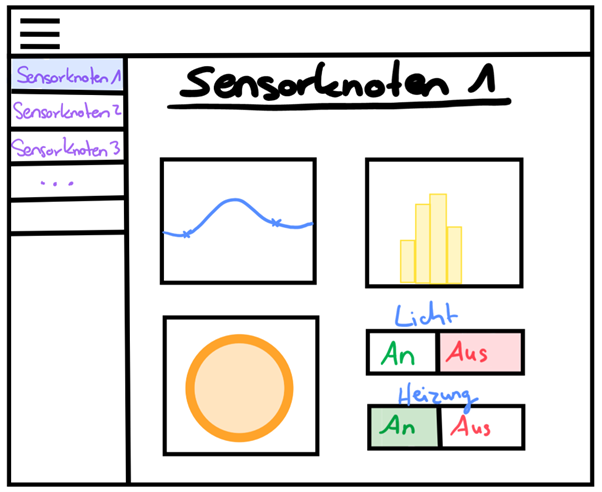
\includegraphics[scale=0.55]{abbildungen/frontend.png}
      \caption{Konzeptzeichnung Frontend}
      \label{fig:frontend}
 \end{figure}
 
Für die Entwicklung am Frontend hat sich Angular als geeignet erwiesen. Da in der Gruppe bereits Erfahrung in diesem vorhanden ist. 
Ngx-admin wird hierbei als Dashboard Template verwendet. 
Es wurde sich für dieses Template entschieden, wegen der modularen Strukturierung, der umfangreichen Dokumentation und der schönen optischen Oberfläche. 
Ngx-admin selbst verwendet die Nebular UI Bibliothek für seine Module.

Abbildung \ref{fig:frontend} zeigt eine Konzeptzeichnung des Frontends. 
Bei der Darstellung sollen die einzelnen Sensorknoten links als Menüpunkte im Navigator angezeigt werden. 
Sollten die Knoten einer Gruppe untergeordnet sein, so ist diese im Navigator erkennbar und der Knoten steht unter einem Gruppen-Menüpunkt. 
Auf der rechten Seite soll das eigentliche Dashboard dargestellt werden. 
Hier befinden sich zum einen Diagramme zur Visualisierung/ Auswertung der Daten und zum anderen Schaltflächen für das Bedienen von Aktoren. 
Bei der Auswahl eines einzelnen Knotens sollen die Daten dieses speziellen Knotens visualisiert werden, bei der Auswahl einer Gruppe soll ein Überblick über die Gruppe gezeigt werden.




\subsection{Gesamtarchitektur}
Abbildung \ref{fig:arch} zeigt einen symbolischen Aufbau der Anwendung.

\begin{figure}[thpb]
      \centering
      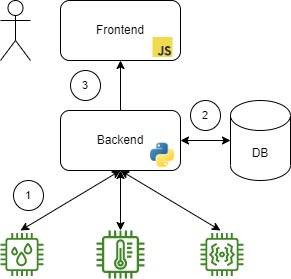
\includegraphics[scale=0.6]{abbildungen/arch.jpeg}
      \caption{Konzept Architektur}
      \label{fig:arch}
 \end{figure}


%%%%%%%%%%%%%%%%%%%%%%%%%%%%%%%%%%%%%%%%%%%%%%%%%%%%%%%%%%%%%%%%%%%%%%%%%%%%%%%%%%%%%%%%%%%%%%
\addtolength{\textheight}{-10cm}   % This command serves to balance the column lengths
                                  % on the last page of the document manually. It shortens
                                  % the textheight of the last page by a suitable amount.
                                  % This command does not take effect until the next page
                                  % so it should come on the page before the last. Make
                                  % sure that you do not shorten the textheight too much.
%%%%%%%%%%%%%%%%%%%%%%%%%%%%%%%%%%%%%%%%%%%%%%%%%%%%%%%%%%%%%%%%%%%%%%%%%%%%%%%%%%%%%%%%%%%%%%

\end{document}
